\section{Motivation: Serialization and Garbage-Collection Costs}

As datasets grow beyond available DRAM, frameworks may offload cached objects to storage.
This reduces the amount of data held in the managed heap, but introduces serialization and deserialization (S/D) work.
A large managed heap avoids some S/D work, but may increase GC work.
This tradeoff is illustrated with two Spark workloads, Linear Regression (LR) and Logistic Regression (LgR), which represent data aggregation and iterative computation, respectively.
Spark caches intermediate results to avoid recomputation across stages.

For this investigation, we vary the portion of heap allocated to execution and on-heap cache.
Spark divides the available heap between memory required for task execution and on-heap memory for cached intermediate results.
The parameter $F=C/H$ specifies the fraction of the heap used as an on-heap cache, where $C$ is cache capacity and $H$ is heap capacity.
$F$ is a soft boundary between zero and one, and either function can use more than its share when the other function does not use its partition.

\begin{figure}[t]
  \centering
  
\includegraphics[width=0.2\linewidth]{teraheap/fig/gc_serdes_leg-crop.pdf}
  \\
  \vspace{-8pt}
  \subfloat[Linear Regression]{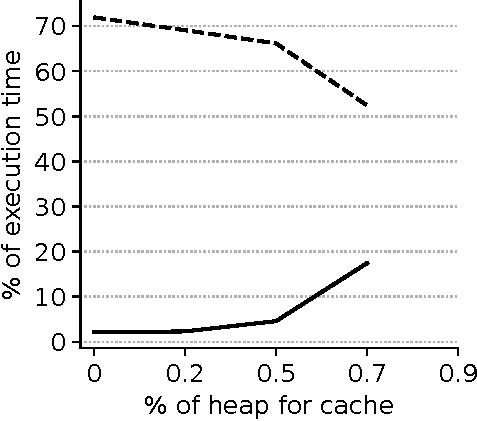
\includegraphics[width=0.3\linewidth]{teraheap/fig/lr_gc_serdes_line-crop.pdf}}
  \hspace{10pt}
  \subfloat[Logistic Regression]{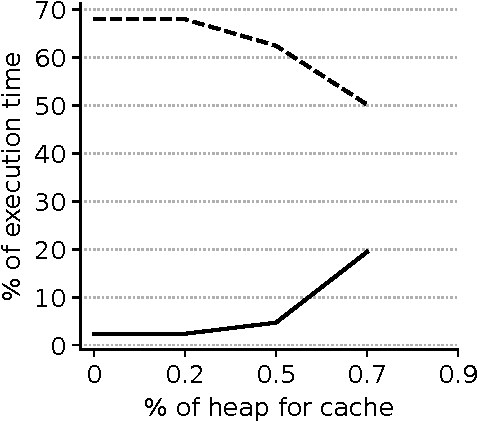
\includegraphics[width=0.3\linewidth]{teraheap/fig/lgr_gc_serdes_line-crop.pdf}}
  \caption{Tradeoff between \teraheapSD and \teraheapGC overhead for (a) Linear Regression and (b) Logistic Regression workloads in Spark.}
  \label{fig:tradeoffs}
\end{figure}

Figure~\ref{fig:tradeoffs} shows the tradeoff between \teraheapGC and \teraheapSD as $F$ varies.
The total heap size in LR and LgR is \SI{64}{GB}.
When $F=0$, Spark serializes and offloads all cached data to storage without keeping cached data on the heap.
In this setting, S/D cost is 24\% and 30\% higher than at $F=0.7$ in LR and LgR, respectively.
At $F=0.7$, GC time increases by 88\% compared with $F=0$ in both workloads.
The larger on-heap cache increases memory pressure and the JVM runs GC more frequently to free space for objects allocated during execution.
